\section{Definitions}

\emph{MAPF instance} $\inst$ is a pair $\inst = (G,A)$, where $G$ is a graph $G = (V,E)$ and $A$ is a set of agents. Each agent $a_i \in A$ is a pair $a_i = (s_i,g_i)$, where $s_i \in V$ is a starting location and $g_i \in V$ is a goal location of agent $a_i$.

Our task is to find a \emph{valid plan} $\pi_i$ for each agent $a_i \in A$ such that it is a valid path from $s_i$ to $g_i$. We use $\pi_i(t) = v$ to denote that agent $a_i$ is located in vertex $v$ at timestep $t$. Time is discrete and at each timestep $t$, an agent can either wait in its current location or move to a neighboring location.

Furthermore, we require that each pair of plans $\pi_i$ and $\pi_j$, $i \neq j$ is collision-free. Based on MAPF terminology~\cite{stern2019mapfVarians}, there are five types of collisions. % (see Figure~\ref{fig:conflict_def}). 
In this work, we forbid \emph{edge}, \emph{vertex}, and \emph{swapping} conflict while allowing \emph{following} and \emph{cycle} conflicts since during the last two conflicts, the agents are not occupying the same physical location. Note however, that all of the proposed methods will work with any other setting as well.%We call this setting \emph{parallel motion}, as opposed to \emph{pebble motion}~\cite{pebble_motion}, where all of the conflicts are forbidden.

%\begin{figure}[ht]
%\centering
%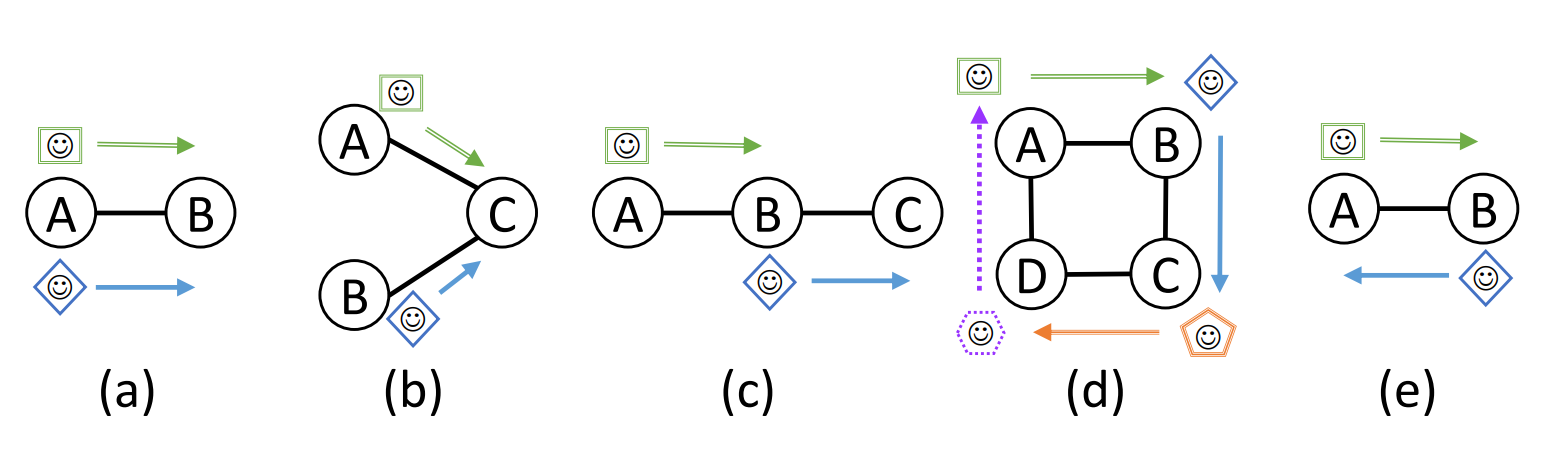
\includegraphics[width=0.99\columnwidth]{img/conflicts.PNG}
%\caption{Conflicts between two or more agents. (a) \emph{edge conflict}, (b) \emph{vertex conflict}, (c) \emph{following conflict}, (d) \emph{cycle conflict}, (e) \emph{swapping conflict}. Figure taken from~\cite{stern2019mapfVarians}.}
%\label{fig:conflict_def}
%\end{figure}

In this paper, we are interested in finding a \emph{makespan} optimal solution. Makespan (or sometimes horizon) is the temporal duration of the plan. Once an agent arrives at its goal location it does not disappear. It may move out of the goal location again, however, the plan ends once all of the agents are at the goal location at the same time. This means that the length of the plan $|\pi_i|$ is the same for all of the agents. Another cost function often used in literature is \emph{sum of costs}~\cite{ICTS_soc}. Note that finding an optimal solution for either of the cost functions is an NP-Hard problem~\cite{NP-hard1,NP-hard2}.